% THIS TEMPLATE IS A WORK IN PROGRESS
% Adapted from an original template by faculty at Reykjavik University, Iceland

\documentclass{scrartcl}
\usepackage{siunitx}
\usepackage[table,xcdraw]{xcolor}

% Adapted from an original template by Hlyni Arnórssyni, Reykjavik University, Iceland
%
% ------------------------------ SETTINGS
\usepackage{geometry}

\geometry{
    paper=a4paper, % Paper size
    top=2.5cm, % Top margin
    bottom=2.5cm, % Bottom margin
    left=2.5cm, % Left margin
    right=2.4cm, % Right margin
    headheight=0.75cm, % Header height
    footskip=1.5cm, % Space from the bottom margin to the baseline of the footer
    headsep=0.75cm, % Space from the top margin to the baseline of the header
%showframe, % Uncomment to show how the type block is set on the page
}

\usepackage{blindtext}
%-------------------------------- Character encoding ----------------------------
\usepackage[T1]{fontenc}
\usepackage[utf8]{inputenc}

%----------------------------- Mathematics packages from AMS ---------------

\usepackage{amsmath, amsfonts, amsthm, amssymb}
\usepackage{braket, nicefrac}

% ----------- International System of Units

%------------------------------ Lists / numbers -------------------------
\usepackage{enumitem, multicol}

%------------------------------- Figure insertions --------------
\usepackage{graphicx, float}  % Use option [H] to force the placement of a figure
\usepackage{keystroke}
\usepackage{pgfplots}\usepgfplotslibrary{units}\pgfplotsset{compat=1.16}

%------------------------------- Line Spacing --------------
\usepackage{setspace}

%------------------------------- Depth of the ToC --------------
\setcounter{tocdepth}{2}

%%%%%%%%%%%%%%%%%%%%%%%%%% Hyperlink References %%%%%%%%%%%%%%%%%%%%%%%%%%%
\usepackage{hyperref}

%--------------------% Storage Path for images %-----------------%
\graphicspath{{graphics/}{Graphics/}{./}}

%%%%%%%%%%%%%%%%%%%%%%%%%% Environments %%%%%%%%%%%%%%%%%%%%%%%%%%%
\renewenvironment{abstract}{
    \begin{center}
        \textbf{Abstract}
        \vspace{0.5cm}
        \par\itshape
        \begin{minipage}{0.8\linewidth}}{\end{minipage}
        \noindent\ignorespaces
    \end{center}
}

\newenvironment{keywords}{
    \begin{center}
        \textbf{Keywords}
        \vspace{0.5cm}
        \begin{minipage}{0.8\linewidth}}{\end{minipage}
        \noindent\ignorespaces
    \end{center}
}

\newenvironment{preface}{
    \begin{center}
        \textbf{Preface}
        \vspace{0.5cm}
        \begin{minipage}{0.8\linewidth}}{\end{minipage}
        \noindent\ignorespaces
    \end{center}
}

\newenvironment{acknowledgements}{
    \begin{center}
        \textbf{Acknowledgements}
        \vspace{0.5cm}
        \begin{minipage}{0.8\linewidth}}{\end{minipage}
        \noindent\ignorespaces
    \end{center}
}



\begin{document}
%Title of the report, name of coworkers and dates (of experiment and of report).
    \begin{titlepage}
        \centering
        
\includegraphics[width=0.6\textwidth]{Graphics/images/bracu_logo}\par
        \vspace{2cm}
        %%%% COMMENT OUT irrelevant lines among the 3 below
        {\scshape\LARGE Department of Computer Science \par}  % if you're a CS major
        {\scshape\LARGE \& \par}                % if have any other major.
        {\scshape\LARGE Engineering \par}      % the name of the other major.
        \vspace{1cm}
        {\scshape\Large CSE422 Project Report\par}
        %{\large \today\par}
        \vfill

        %%%% PROJECT TITLE
        {\huge\bfseries Spam Email Detection\par}
        \vfill

        %%%% AUTHOR(S)
        {\Large\itshape ATHAR NOOR MOHAMMAD RAFEE\\ ID: 20101396 \\ LAB SECTION: 09\\ GROUP: 08}\par
        \vspace{1.5cm}

        \vfill
        supervised by\par
        %%%% SUPERVISOR(S)
        Ms. Afia Fairoose Abedin \& Ms. Sumaiya Akter


        \vfill
% Bottom of the page
    \end{titlepage}


    \newpage



    \doublespacing
    \tableofcontents
    \singlespacing

    \newpage

    \doublespacing


    \section{INTRODUCTION}\label{sec:introduction}
    In, today's ever evolving modern and busy world email is a simple yet very important source
of communication between various groups of people due to personal, business, corporate
and government use-cause reasons.
Over the past few years, the usages of email have greatly increased as
the internet has revolutionized many parts of the world.
Unfortunately, as the number of email users increases, \textbf{SPAM}(also known as junk email)
email targeting general users also increases.
These \textbf{SPAM} emails, which are being sent to numerous recipients, are identical in
nature and being very annoying, they pose various security vulnerabilities to the
client's device if not handled properly.
Apart from that, these \textbf{SPAM} emails take away a lot of precious time from the user
and cause financial loss to corporations and businesses.
To prevent that and make efficient use of emails, in this project I
used various text mining strategies to extract meaningful information from
emails text and used various machine learning algorithms to figure out which one is optimal to
use for spam email detection in common day-to-day life scenarios.


    \section{LEARNING DATA}\label{sec:learning-data}
    The dataset that I used for this project from kaggle\cite{spam-email-detection-dataset}
is called \textbf{\textit{spam email detection dataset}}, and it’s a raw.
The initial data set of was \textbf{5730} rows and \textbf{110} columns,
and many of the columns were not necessary for further use cases.
The first thing I had to do was preprocess the dataset and took it to
a usable state for further text processing and tokenization/word frequency count.


    \section{DATA PREPROCESSING}\label{sec:data-preprocessing}
    As the dataset had a lot of \verb|null| columns and cells, first resolved that issue by dropping the \textbf{null} columns.
After then moved on the \verb|null/NaN| cell and took care of it as well by dropping the null/NaN rows.
Did the necessary encoding(binary label encoding where 0 means non-spam and 1 means spam) for the label and got rid of duplicates values from rows.
After performing these series of data-preprocessing steps, I ended up with \textbf{5693} rows and \textbf{2} columns.
However, converting the plain raw email texts into features was yet to be done.
To achieve this, I used two slightly different text \verb|vectorizer/tokenizer|\textit{(count the frequency of words in texts ignoring some common stop words that have no significant impact on the meaning of the sentences but appear frequently)}\cite{countvectorizer_in_nlp_2020}
namely \verb|CountVectorizer()| and \verb|TfidfVectorizer()| to convert them into features so that later I can train and test various models on them.
After preprocessing the dataset, the dataset contained around \textbf{37000}) features or words\textit{(tokens)} found by \verb|CountVectorizer()| and \verb|TfidfVectorizer()|.
To get an idea about each set of features, I used \verb|wordcloud| to generate visual representations of the most frequently occurring words shown in the below Figure~\ref{fig:cout_vect} and Figure ~\ref{fig:tfidf_vect}.

\begin{figure}[H]
    \begin{center}
        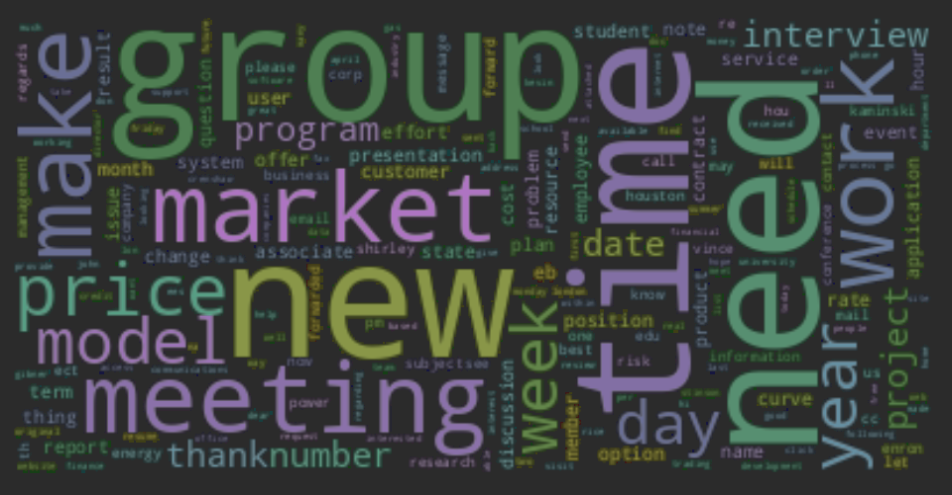
\includegraphics[scale=0.4]{Graphics/images/count_vect}
    \end{center}
    \caption{Frequent Words Found Using count vectorizer}
    \label{fig:cout_vect}
\end{figure}

\begin{figure}[H]
    \begin{center}
        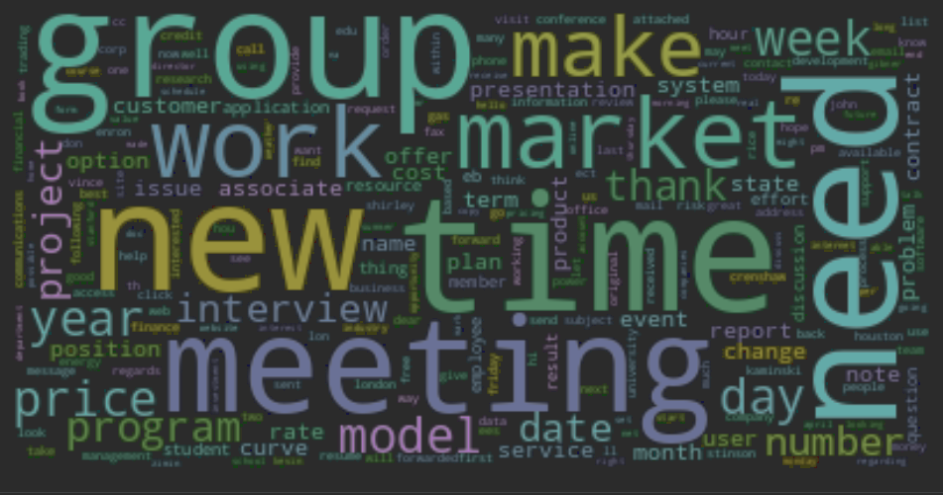
\includegraphics[scale=0.4]{Graphics/images/tfid_vect}
    \end{center}
    \caption{Frequent Words Found Using tfidf vectorizer}
    \label{fig:tfidf_vect}
\end{figure}


    \section{Experimental Result}\label{sec:experimental-result}
    I used the training data obtained from both of the vectorizers(\verb|CountVectorizer()| \& \verb|TfidfVectorizer()|) to train a variety of models using training data and then used testing data to measure various matrices regarding that particular model, most importantly the \textbf{accuracy}.
In order to obtain different metrics regarding a particular model, I used the \verb|classification_report()| method imported from \verb|sklearn.metrics|.

\subsection{Results}\label{subsec:results}
Below, I am attaching all the metrics found by different learning models.

Logistic Regression using \verb|CountVectorizer|
\begin{table}[H]
    \begin{tabular}{lllll}
        & precision & recall & f1-score                     & support \\
        NON-SPAM          & 0.99      & 0.99   & 0.99                         & 843     \\
        SPAM              & 0.98      & 0.97   & 0.98                         & 296     \\
        &           &        &                              &         \\
        \textbf{accuracy} &           &        & \cellcolor[HTML]{FFCCC9}0.99 & 1139
    \end{tabular}\label{tab:Logistic_count_vect}
\end{table}

Logistic Regression using \verb|TfidfVectorizer|
\begin{table}[H]
    \begin{tabular}{lllll}
        & precision & recall & f1-score                     & support \\
        NON-SPAM          & 0.97      & 0.99   & 0.98                         & 843     \\
        SPAM              & 0.96      & 0.91   & 0.93                         & 296     \\
        &           &        &                              &         \\
        \textbf{accuracy} &           &        & \cellcolor[HTML]{FFCCC9}0.96 & 1139
    \end{tabular}\label{tab:Logistic_tfidf_vect}
\end{table}

MultinomialNB using \verb|CountVectorizer|
\begin{table}[H]
    \begin{tabular}{lllll}
        & precision & recall & f1-score                     & support \\
        NON-SPAM          & 1.00      & 0.99   & 0.99                         & 843     \\
        SPAM              & 0.97      & 0.99   & 0.98                         & 296     \\
        &           &        &                              &         \\
        \textbf{accuracy} &           &        & \cellcolor[HTML]{FFCCC9}0.99 & 1139
    \end{tabular}\label{tab:Multinomial_count_vect}
\end{table}

MultinomialNB using \verb|TfidfVectorizer|
\begin{table}[H]
    \begin{tabular}{lllll}
        & precision & recall & f1-score                     & support \\
        NON-SPAM          & 0.83      & 1.00   & 0.91                         & 843     \\
        SPAM              & 1.00      & 0.43   & 0.60                         & 296     \\
        &           &        &                              &         \\
        \textbf{accuracy} &           &        & \cellcolor[HTML]{FFCCC9}0.85 & 1139
    \end{tabular}\label{tab:Multinomial_tfidf_vect}
\end{table}
For some reason there is a lot of difference in terms of accuracy between \verb|Count & Tfidf| Vectorizer when
using Multinomial Naive Bayes Model.


BernoulliNB using \verb|CountVectorizer|
\begin{table}[H]
    \begin{tabular}{lllll}
        & precision & recall & f1-score                     & support \\
        NON-SPAM          & 0.98      & 0.99   & 0.99                         & 843     \\
        SPAM              & 0.97      & 0.95   & 0.96                         & 296     \\
        &           &        &                              &         \\
        \textbf{accuracy} &           &        & \cellcolor[HTML]{FFCCC9}0.98 & 1139
    \end{tabular}\label{tab:BernoulliNB_count_vect}
\end{table}

BernoulliNB using \verb|TfidfVectorizer|
\begin{table}[H]
    \begin{tabular}{lllll}
        & precision & recall & f1-score                     & support \\
        NON-SPAM          & 0.98      & 0.99   & 0.99                         & 843     \\
        SPAM              & 0.97      & 0.95   & 0.96                         & 296     \\
        &           &        &                              &         \\
        \textbf{accuracy} &           &        & \cellcolor[HTML]{FFCCC9}0.98 & 1139
    \end{tabular}\label{tab:BernoulliNB_tfidf_vect}
\end{table}

GaussianNB using \verb|CountVectorizer|
\begin{table}[H]
    \begin{tabular}{lllll}
        & precision & recall & f1-score                     & support \\
        NON-SPAM          & 0.96      & 0.99   & 0.97                         & 843     \\
        SPAM              & 0.97      & 0.87   & 0.91                         & 296     \\
        &           &        &                              &         \\
        \textbf{accuracy} &           &        & \cellcolor[HTML]{FFCCC9}0.96 & 1139
    \end{tabular}\label{tab:GaussianNB_count_vect}
\end{table}

GaussianNB using \verb|TfidfVectorizer|
\begin{table}[H]
    \begin{tabular}{lllll}
        & precision & recall & f1-score                     & support \\
        NON-SPAM          & 0.95      & 0.99   & 0.97                         & 843     \\
        SPAM              & 0.98      & 0.86   & 0.92                         & 296     \\
        &           &        &                              &         \\
        \textbf{accuracy} &           &        & \cellcolor[HTML]{FFCCC9}0.96 & 1139
    \end{tabular}\label{tab:GaussianNB_tfidf_vect}
\end{table}

DecisionTreeClassifier using \verb|CountVectorizer|
\begin{table}[H]
    \begin{tabular}{lllll}
        & precision & recall & f1-score                     & support \\
        NON-SPAM          & 0.96      & 0.97   & 0.97                         & 843     \\
        SPAM              & 0.92      & 0.89   & 0.91                         & 296     \\
        &           &        &                              &         \\
        \textbf{accuracy} &           &        & \cellcolor[HTML]{FFCCC9}0.95 & 1139
    \end{tabular}\label{tab:DecisionTreeClassifier_count_vect}
\end{table}

DecisionTreeClassifier using \verb|TfidfVectorizer|
\begin{table}[H]
    \begin{tabular}{lllll}
        & precision & recall & f1-score                     & support \\
        NON-SPAM          & 0.96      & 0.97   & 0.97                         & 843     \\
        SPAM              & 0.92      & 0.89   & 0.91                         & 296     \\
        &           &        &                              &         \\
        \textbf{accuracy} &           &        & \cellcolor[HTML]{FFCCC9}0.95 & 1139
    \end{tabular}\label{tab:DecisionTreeClassifier_tfidf_vect}
\end{table}

\subsection{Analysis}\label{subsec:analysis}
All of the used models have more or less the same outcome excluding Multinomial Naive Bayes~\ref{tab:GaussianNB_tfidf_vect} model
where we see a significant difference between two vectorizers.
Below is the accuracy barchart using \verb|CountVectorizer()|\ref{fig:cout_vect_acc_chart} and for \verb|TfidfVectorizer()|\ref{fig:tfidf_vect_acc_chart}.

\begin{figure}[H]
    \begin{center}
        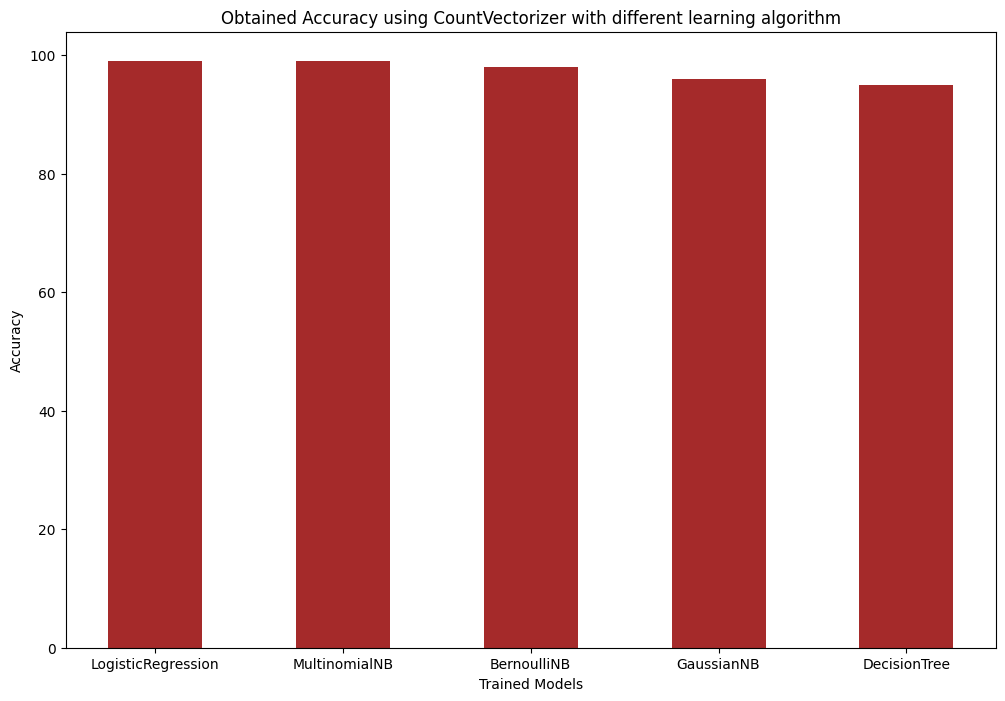
\includegraphics[scale=0.4]{Graphics/chart/count_vect}
    \end{center}
    \caption{Accuracy using count vectorizer for different Models}
    \label{fig:cout_vect_acc_chart}
\end{figure}

\begin{figure}[H]
    \begin{center}
        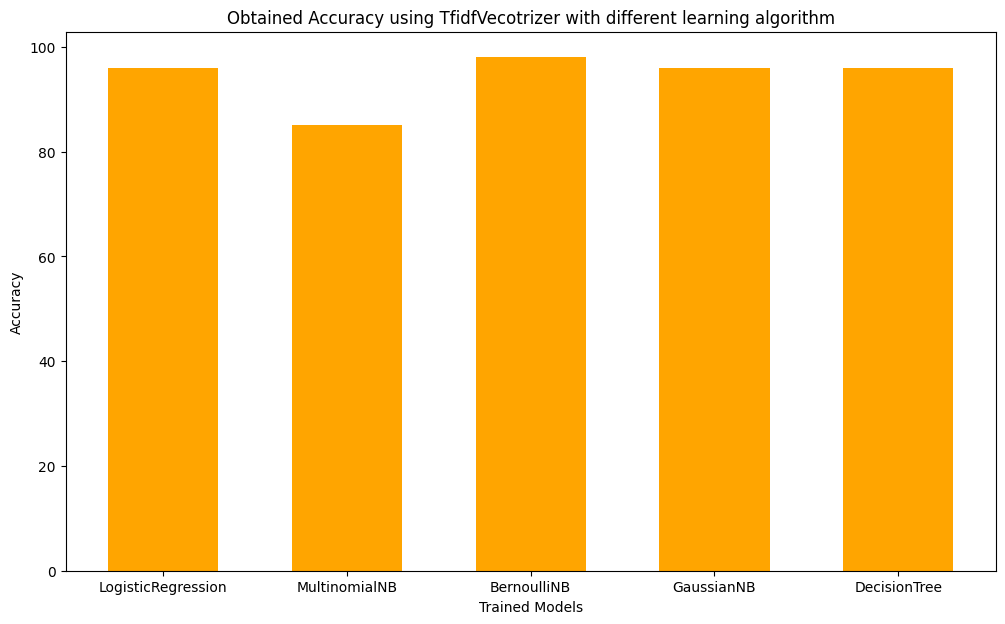
\includegraphics[scale=0.4]{Graphics/chart/tfidf_vect}
    \end{center}
    \caption{Accuracy using tfidf vectorizer for different Models}
    \label{fig:tfidf_vect_acc_chart}
\end{figure}

From the above graph we can see, except for one model, both tokenizers are equivalent and they are quite accurate in terms of detection
spam and non-spam email regardless of the model.



    \section{Conclusion}\label{sec:conclusion}
    
In the end, the use of machine learning techniques for spam email detection has proven to be an effective way to automatically filter out unwanted messages.
And to do so, we don't need to use advanced methods such as 10-level deep neural networks;
 instead, a simple Logistic Regression is way more than enough to detect 98\% of the time.
By training a model on a large dataset of labeled emails, we were able to achieve high levels of accuracy in predicting whether a given email was spam or not.
The ability to accurately identify and remove spam emails not only helps to protect individuals from potential scams and phishing attempts,
but also helps to reduce the overall amount of spam that is sent and received, making the internet a safer and more efficient place.
Overall, this project has demonstrated the power of machine learning in the fight against spam email.
\newpage
\singlespacing
\bibliographystyle{IEEEtran}
\bibliography{main}


%------ To create Appendix with additional stuff -------%
%\newpage
%\appendix
%\section{Appendix}
%Put data files, CAD drawings, additional sketches, etc.

\end{document}
